\section{Empirical Performance}
\label{sec:experiments}
% Experimental results

% Things to be tested
We evaluated the options defined using our method on the Taxi domain described
in \secref{sec:approach}. We compared the performance of Macro Q learning and
Intra-option Q-learning agents using the following option schemes,
\begin{itemize}
   \item \textbf{Small World} Options were generated randomly connecting two nodes of
       the domain using an inverse square law, as described in
       \secref{sec:approach}, with $r = 2$.
   \item \textbf{Betweenness} Options were generated to take any node to a local maxima
       of the betweenness function.
   \item \textbf{Random} Options were generated by randomly connecting two nodes in the
       domain.
   \item \textbf{Manual} Options were manually defined to take the taxi to one of the
       four pads by the shortest path.
   \item \textbf{None} No options were used.
\end{itemize}

The Intra-option Q-learning algorithm requires that the option policies
themselves be Markov, require that every state that the option can visit be part
of $\initset$. For the experiments using the Intra-option learning algorithm, we
modified the ``Small World'' options slightly such that all nodes along the path
were in the initiation set of the option as well.

% Experimental Parameters
To compare the different approaches, we measuring the ratio of how long the taxi
takes to complete the task to the shortest time possible to complete the task,
and have termed this measure "optimality".  Each experiment was averaged over
$200$ runs, and run for $1500$ episodes. We set $\alpha$ to $0.8$ for all the
experiments. We ran the experiments for two values of $\gamma$, $0.90$ and
$0.99$, with equal performance. We present the results only for $\gamma$ set to
$0.99$.

We plotted the value of optimality versus the number of episodes of the agent,
and have also zoomed into the later episodes to have a closer look at the
converged behaviour.

% Plots
\begin{figure}[ht]
    \centering
    \subfigure[]{
    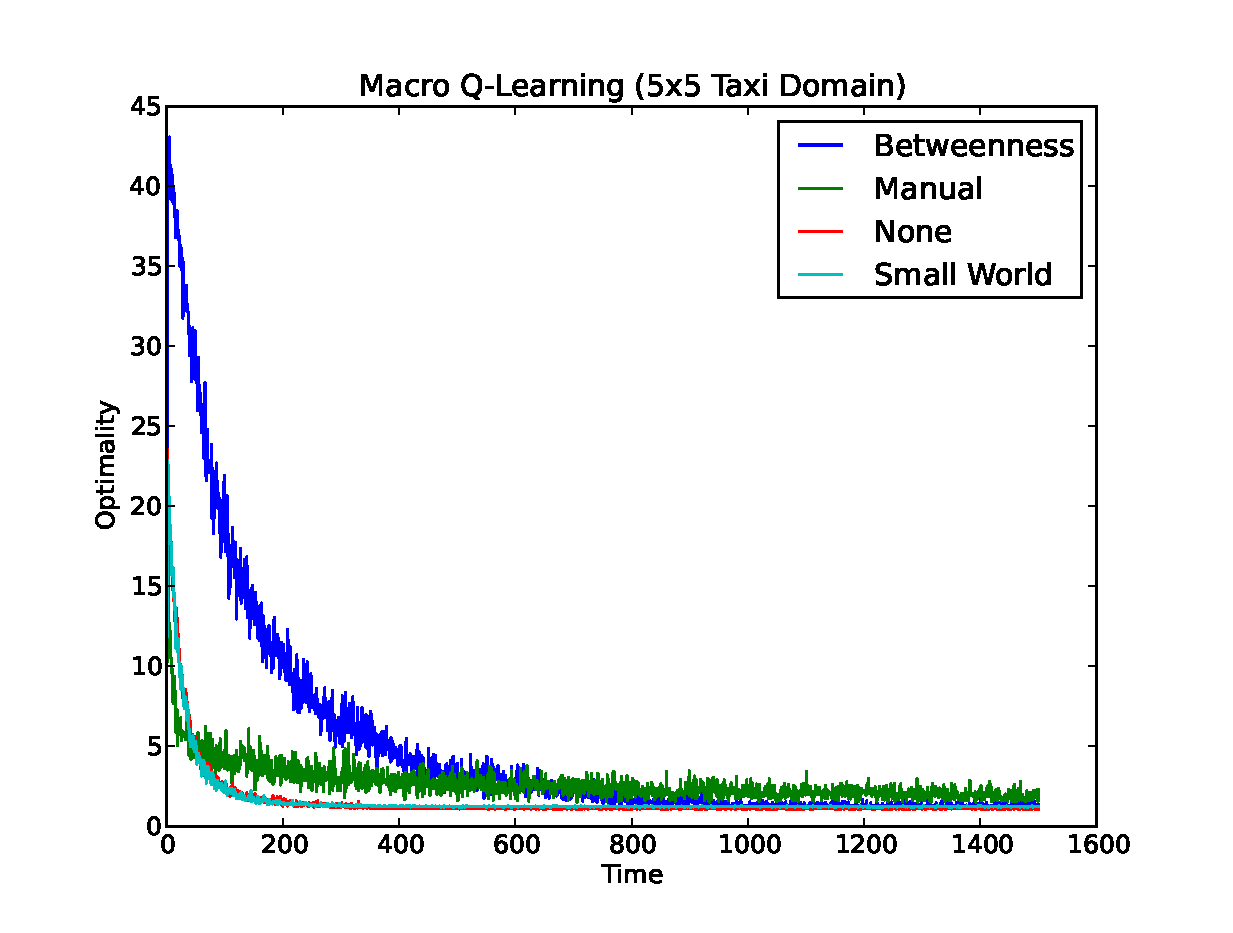
\includegraphics[width=4in]{figures/MacroQ-0_99-taxi1}
    }
    \subfigure[]{
    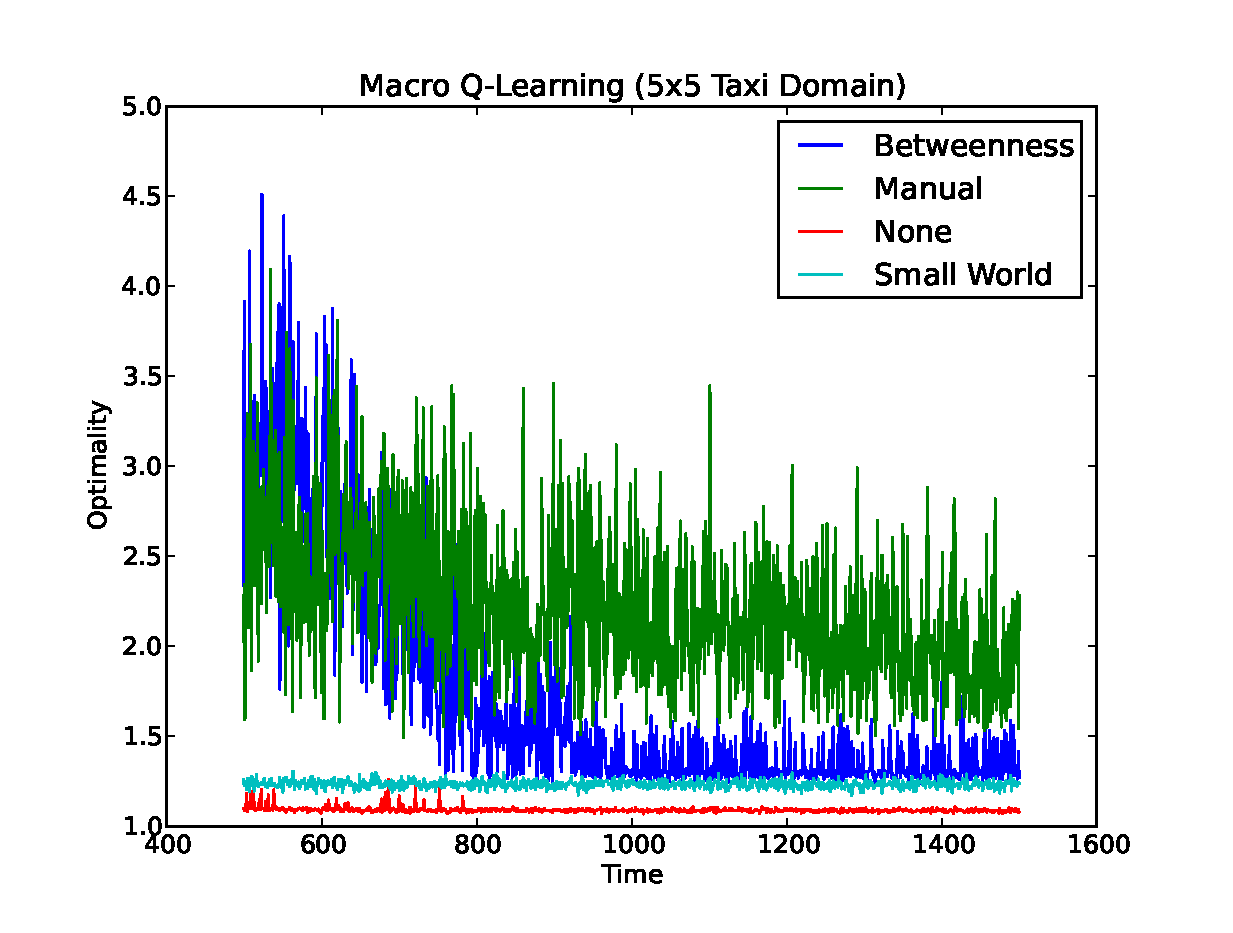
\includegraphics[width=4in]{figures/MacroQ-0_99e-taxi1}
    }
    \caption{Macro Q-learning using 20 options }
    \label{fig:MacroQ-0.99}
\end{figure}

\begin{figure}[ht]
    \centering
    \subfigure[]{
    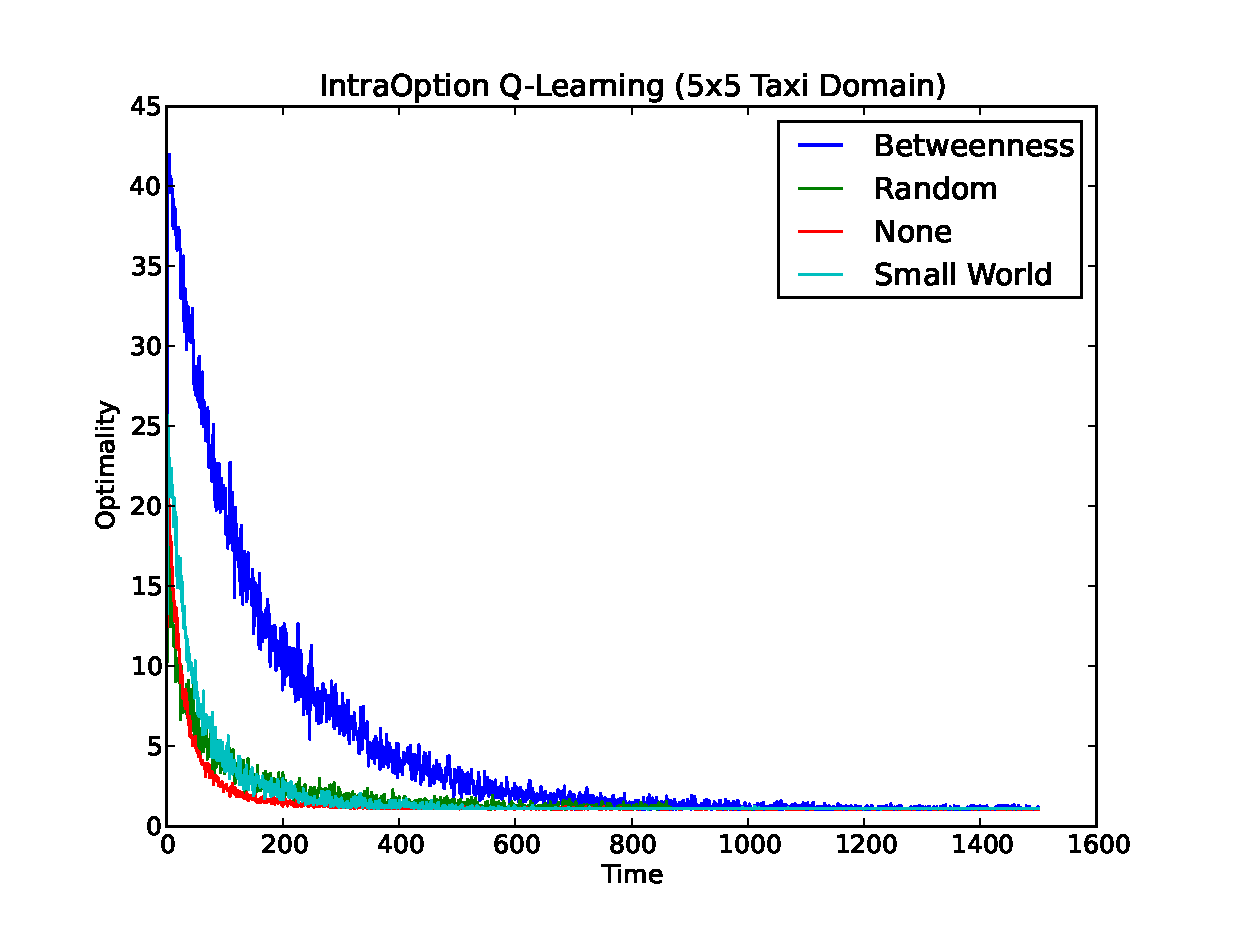
\includegraphics[width=4in]{figures/IntraQm-0_99-taxi1}
    }
    \subfigure[]{
    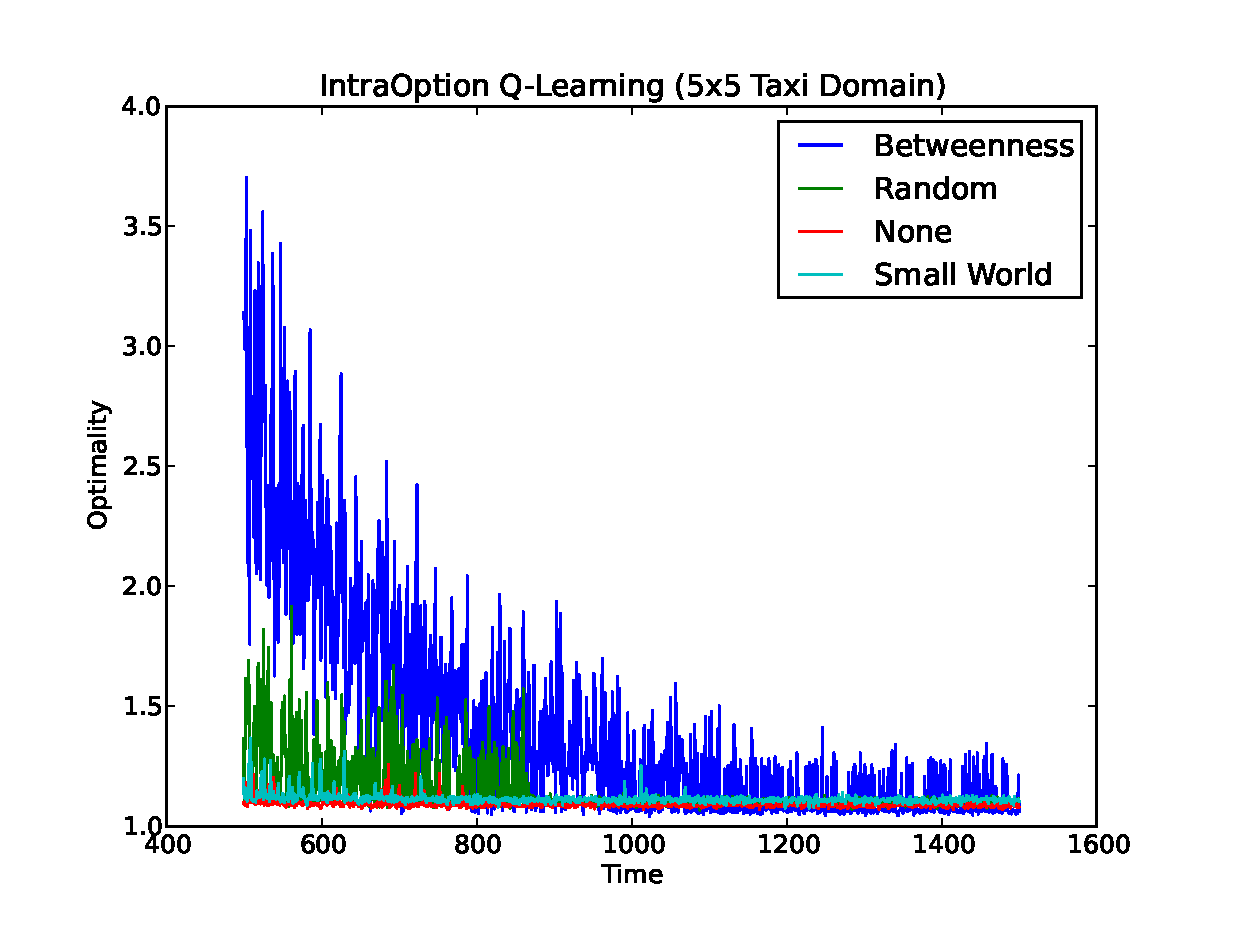
\includegraphics[width=4in]{figures/IntraQm-0_99e-taxi1}
    }
    \caption{Intra-option Q-learning using 20 options }
    \label{fig:IntraQ-0.99}
\end{figure}

\begin{figure}[ht]
    \centering
    \subfigure[]{
    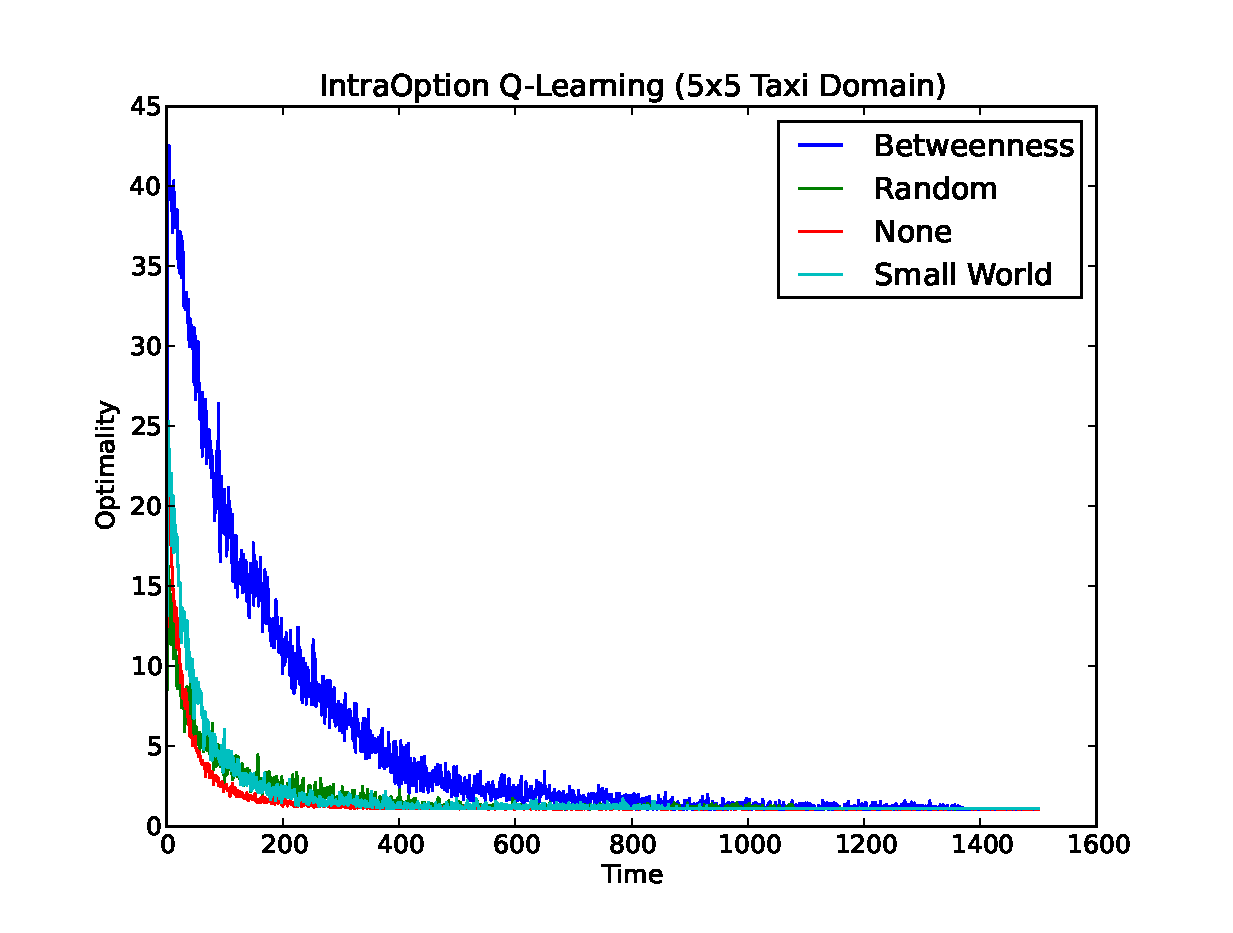
\includegraphics[width=4in]{figures/IntraQm-0_99-50-taxi1}
    }
    \subfigure[]{
    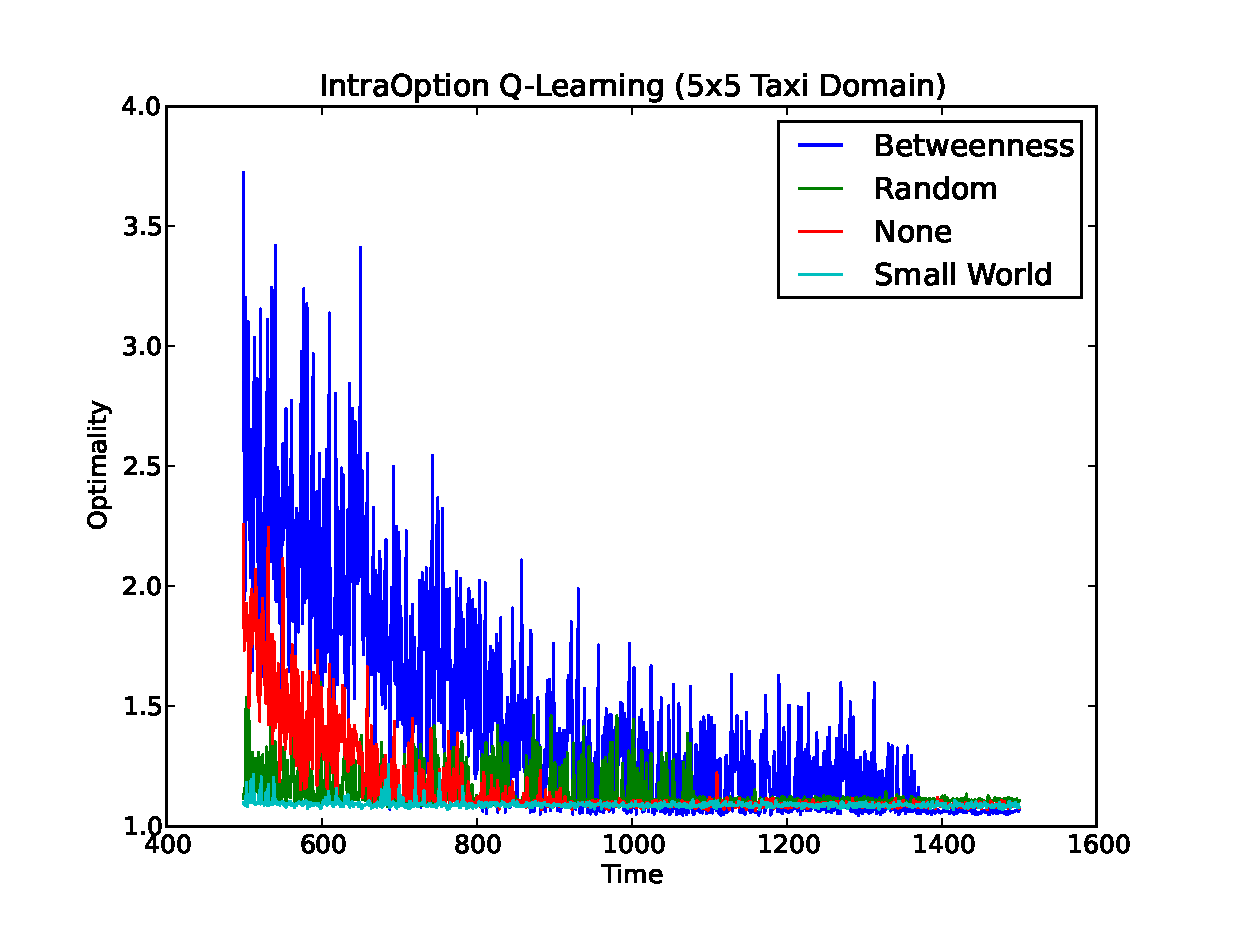
\includegraphics[width=4in]{figures/IntraQm-0_99e-50-taxi1}
    }
    \caption{Intra-option Q-learning, using 50 options }
    \label{fig:IntraQ-0.99-50}
\end{figure}

% Brief on results
We note that the agents using Small World options converge quickly to the
optimal value (i.e. 1), and have small variance. Expectedly, the performance
using Intra-option Q-learning (\autoref{fig:IntraQ-0.99}) is significantly
better than Macro Q-learning (\autoref{fig:MacroQ-0.99}). The performance of
small world options does not significantly differ between using 20 options
(\autoref{fig:IntraQ-0.99}) or 50 options (\autoref{fig:IntraQ-0.99-50}).

We find it surprising that betweenness performs worse than the remaining
schemes. Our options differ from the random options defined in \cite{Simsek} as
we select random paths instead of random nodes to which all other nodes are
connected. As a result, for many nodes there are few if any options. As adding
options also increases the number of actions that an agent can choose from, this
might have lead to the better performance of Random and Small World, which are
both path-based options.

% \begin{table}[ht]
%     \centering
%     \begin{tabular}{ r | r }
%           &  \\ \hline
%           &  \\
%     \end{tabular} 
%     \caption{ }
%     \label{tbl:rtt-summary}
% \end{table}

% \begin{figure}[s]
%     \centering
%     \includegraphics[width=5in]{filename}
%     \caption{ }
%     \label{fig:high-variance-rtt}
% \end{figure}

